% https://www.sciencedirect.com/book/9780128042045/wheeled-mobile-robotics
Path planning is the task of finding a continuous path from the start to the goal. The path planning algorithm must have a definiton of an executable path and a goal. The start is stated by the current position of the \acs{uav}. The algorithm receives a occupancy grid and returns the shortest path from start to goal. \cite{KLANCAR2017161}

% https://www.gamedev.net/tutorials/programming/general-and-gameplay-programming/introduction-to-octrees-r3529/
The occupancy grid is obtained as the output of \acs{rtabmap} and is represented in an Octree format. An Octree is a special type of subdividing tree in a \acs{3d} space. One node in an Octree can be subdivided into eight smaller nodes, each node represents a free or occupied space. \cite{octrees_gamedev}

\begin{figure}[!h]
  \centering
  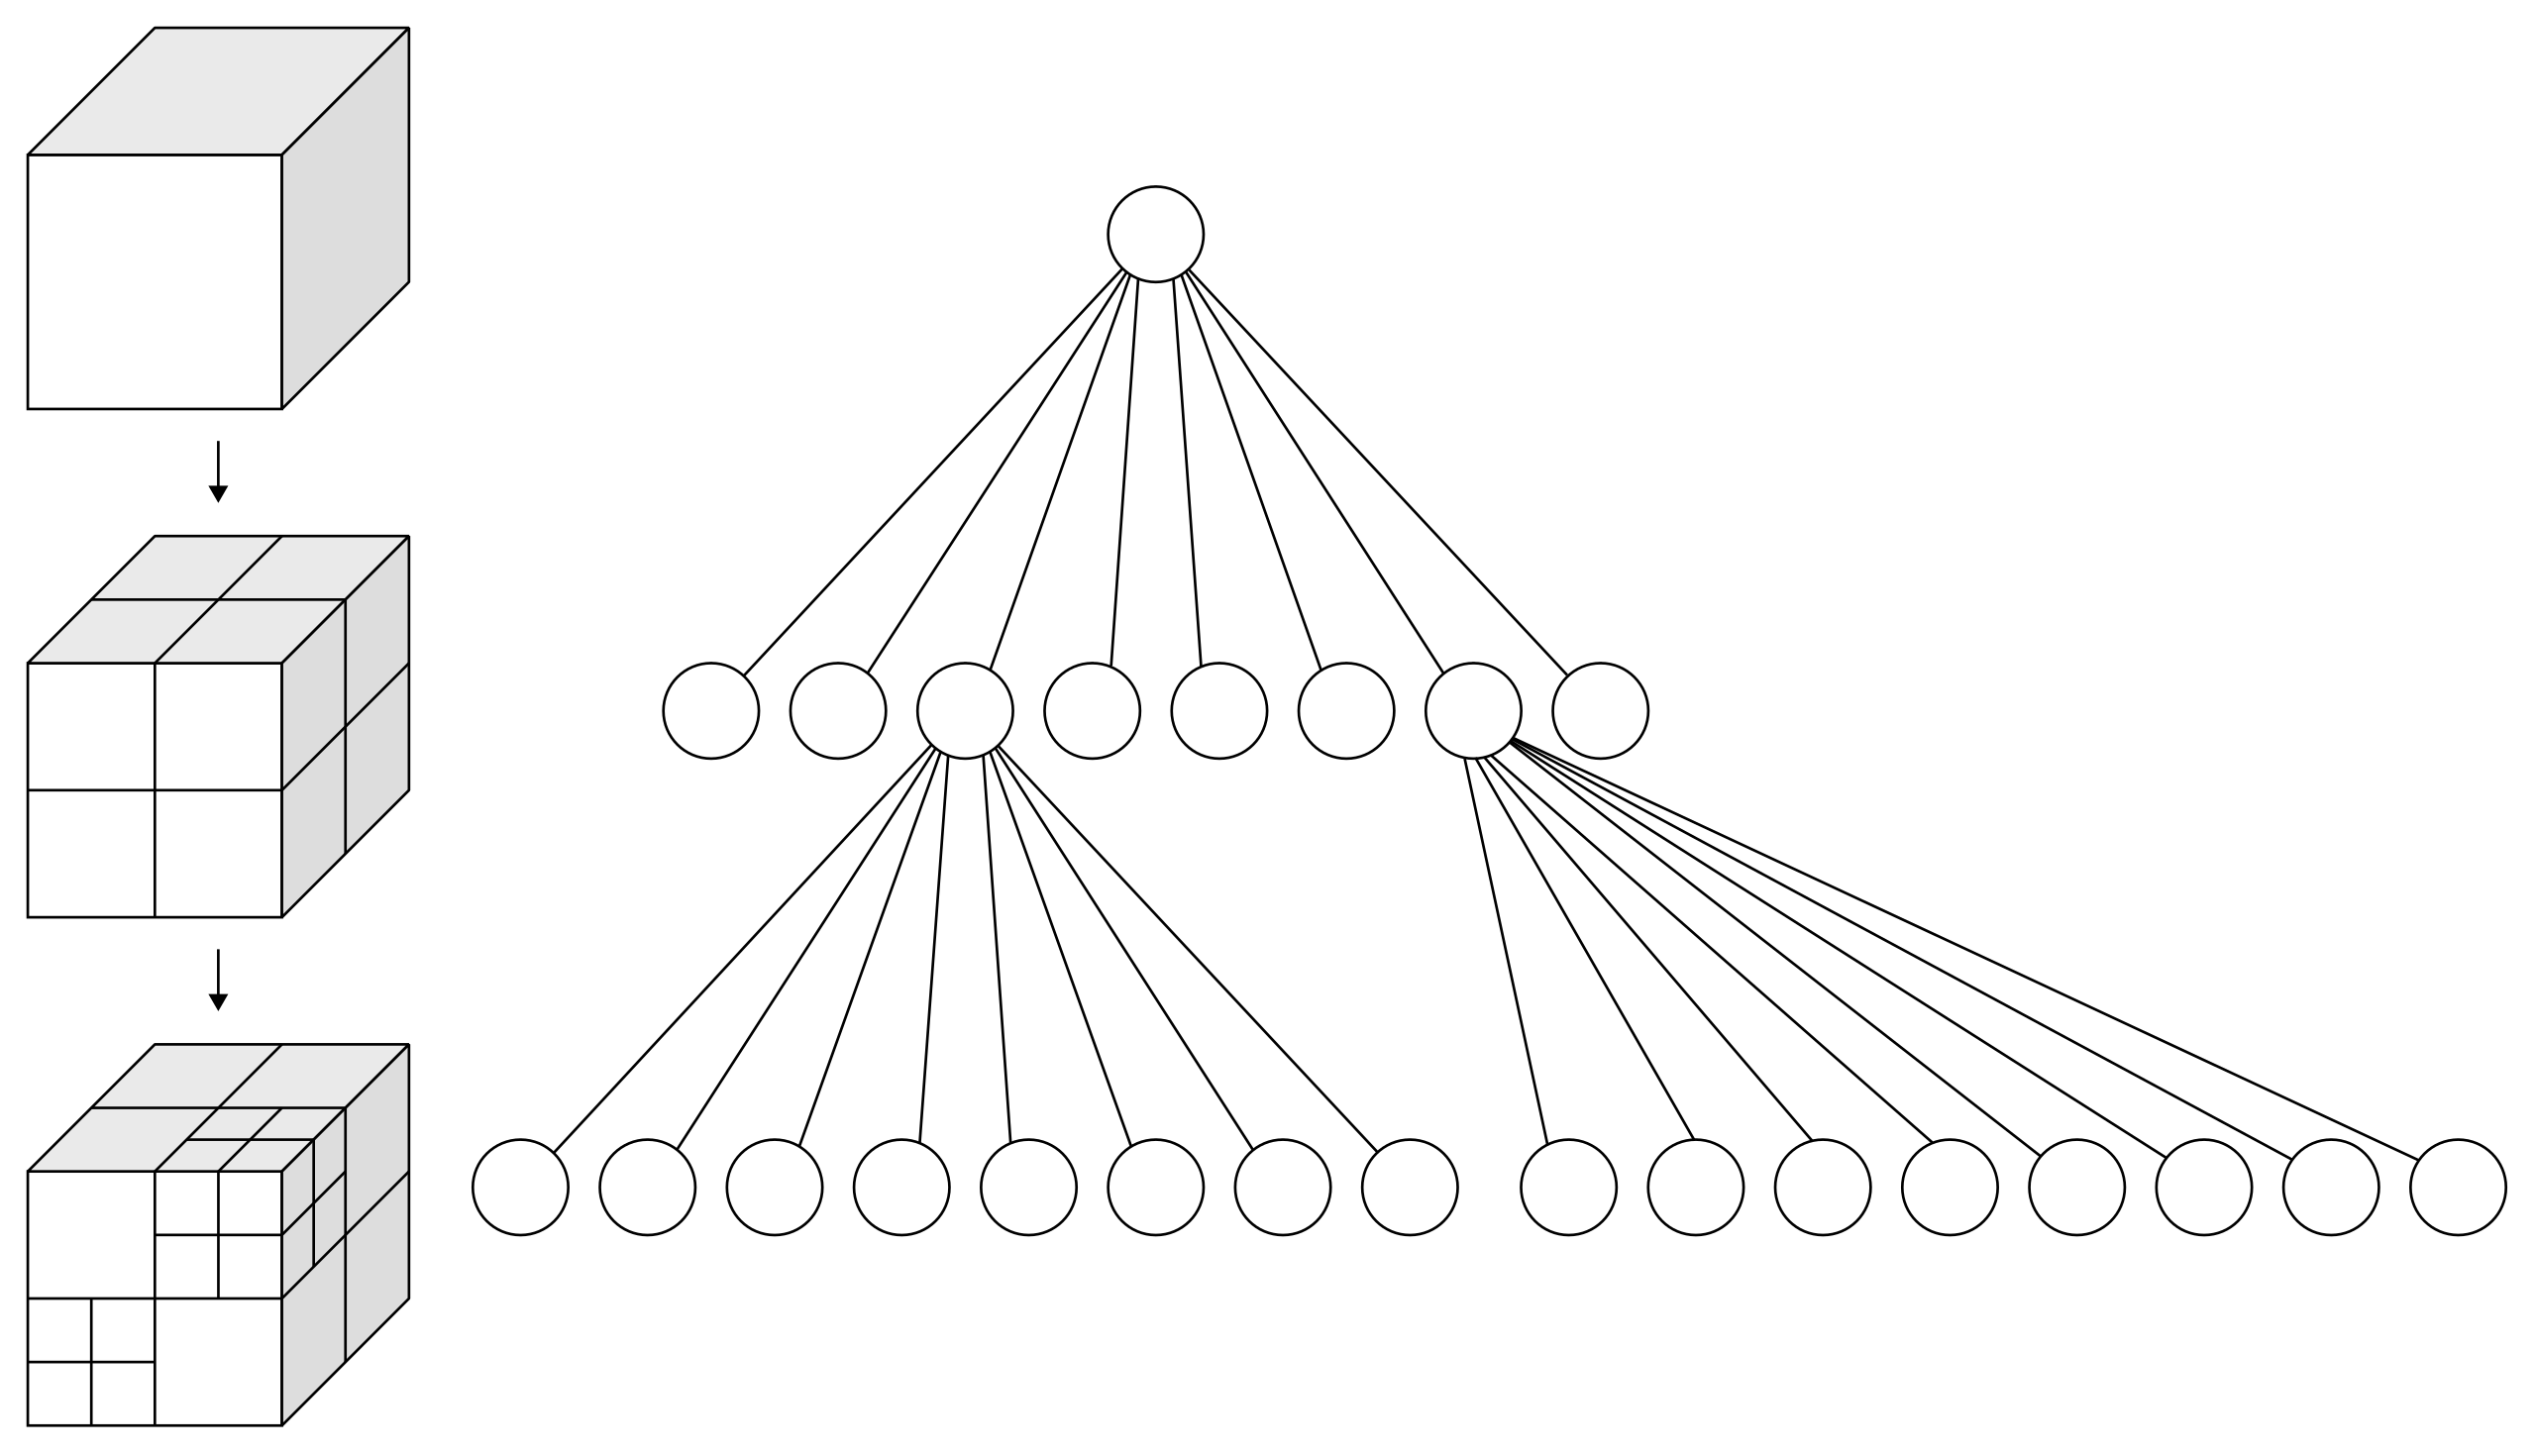
\includegraphics[width=0.6\linewidth]{images/octree.png}
  \caption{Octree \cite{octrees_gamedev}}
\end{figure}